\documentclass[10pt]{beamer}

\usetheme[progressbar=frametitle]{metropolis}
\usepackage{appendixnumberbeamer}

\usepackage{booktabs}
\usepackage[scale=2]{ccicons}

\usepackage{pgfplots}
\usepgfplotslibrary{dateplot}

\usepackage{xspace}
\newcommand{\themename}{\textbf{\textsc{metropolis}}\xspace}

\title{Adversarial Attacks}
\subtitle{Software Design Document}
% \date{\today}
\date{}
\author{\\Adhithya S.\\Janaki Keerthi\\Jayasoorya Jithendra\\Jessal V. A.\\\\\\under the guidance of Prof. Rajasree R.}

%\institute{under the guidance of Prof. Rajasree R.}
% \titlegraphic{\hfill\includegraphics[height=1.5cm]{logo.pdf}}

\begin{document}

\maketitle

\begin{frame}{Table of contents}
  \setbeamertemplate{section in toc}[sections numbered]
  \vspace{0.51in}
  \tableofcontents
\end{frame}

\section{Introduction}

\begin{frame}{Introduction}
\begin{itemize}
\item An adversarial attack consists of subtly modifying an image in such a way that the changes are
almost undetectable to the human eye.
\item The modified image
is called an adversarial image, and when submitted to a
classifier is misclassified, while the original one is correctly
classified.
\item The real-life applications of such attacks can be
very serious, eg., one could modify a traffic sign to
be misinterpreted by an autonomous vehicle, and cause an
accident.
\end{itemize}
  
\end{frame}

\section{Motivation}

\begin{frame}{Motivation}
\begin{itemize}
    \item Deep Neural Networks are susceptible to adversarial noise.
\item The motivation behind the project is to make use of this vulnerability in a constructive manner in order to improve computer security.
\item Adversarial examples for captcha applications are very difficult for Deep Learning algorithms while easy for humans (adversarial noise tends to be small and does not affect human perception of image
content).
\end{itemize}
	
\end{frame}

\section{Problem Definition}
\begin{frame}{Problem Definition}
    \begin{itemize}   
    \item The Internet is a place that requires security, privacy and equality.\\\bigskip
    \item With the AI bots becoming more and more intelligent nowadays, they are able to automate test to distinguish a human and a bot. 
    \item This can lead to the bots getting faster request reply from the web server, thus giving some users advantage over others.
    \item This can also lead to bots performing DDoS(Distributed Denial of Service) attacks easily on Web Servers as CDN(Content Delivery Networks) use captcha to distinguish bots and humans.\\\bigskip
    
    \item While AI bots have grown exponentially better in face recognition, this can be a privacy breach as a user might not want his or her face recognized in a photo.
    
    \end{itemize}
\end{frame}


\section{Problem Description}
\begin{frame}{Problem Description}
\begin{itemize}
    \item Captchas are traditionally defined as
automatically constructed problems, that are very difficult
to solve for AI algorithms, but easy for humans.
\item  Due to the
fast progress in AI, an increasing number of captcha
designs have become ineffective, as the underlying AI
problems have become solvable by algorithmic tools.
\item The susceptibility of DNNs to adversarial attacks can thus be used constructively in order to prevent bots from automating captcha tests.
\end{itemize}

\end{frame}


\section{Objectives}
\begin{frame}{Objectives}
    
    \item To perform adversarial attacks on Image captchas to prevent bots from automating captcha tests.
    \item To perform adversarial attacks on Human Images to prevent face recognition. 
    

\end{frame}

\section{Literature Review}
\begin{frame}{Why Adversarial Attacks work?}
    
    \begin{itemize}
        \item Modern hardware manipulate images as 8 bit values.
        \item Modern Neural Networks manipulate data in 32 bit floating point numbers.
        \item Thus Adversarial Attacks manipulate the data such that the main 8 bits are unchanged, by modifying the remaining 24 bits.
    \end{itemize}
      
\end{frame}

\begin{frame}{Where Modern Neural Networks fail?}
    
    \begin{itemize}
       \item  Neural Networks perform linear transformation to the matrices.
       \item  Additions of dropout, pre-training, and model averaging do not improve the model’s vulnerability to adversarial examples.
       \item Convolutional neural networks approximates Perceptual distance as Euclidean distance.
       \item This resemblance is clearly flawed if images that have an
        immeasurably small perceptual distance correspond to completely different classes in the network’s representation.
     \end{itemize}   

\end{frame}

\begin{frame}{The Linear Explanation of Adversarial Examples}
        The precision of the features is limited.\\\bigskip
        It is not rational for the classifier to respond differently to an input x than to an adversarial input $ x~ = x + \eta$  if every element of the perturbation $\eta$ is smaller than the precision of the features.\\\bigskip
        Precision of the features is about (1/256) $\approx$ (0.03).
        Thus for $\eta \leq (0.03)$ the adversarial input should act similiar to the original input.\\\bigskip
        
        Thus effectively the transformation becomes:\\
        {$$ W^{T}*\widetilde{x} = W^{T}*x + W^{T}*\eta $$}
\end{frame}

\begin{frame}{Fast Gradient Sign Method}
        
        FGSM computes an adversarial image by adding a pixel-wide perturbation of magnitude in the direction of the gradient. This perturbation is computed with a single step, thus is very efficient in terms of computation time.\\
        
        {$$ X^{adv} = x + \epsilon . sign(\nabla_{x}J(x, y_{true}))$$}\\\bigskip
        
        \begin{flushleft}
        where,\\
        X : is the clean input\\
        $X^{adv}$ : is the perturbed adversarial example.\\
        J : is the classifier's loss function.\\
        $y_{true}$ : is the true label for the input x.\\
        \end{flushleft}
        
\end{frame}

\begin{frame}{Targeted and Iterative Fast Gradient Sign Method}
        
        \textbf{Targeted Fast Gradient Sign Method}
        Similarly to the FGSM, in this method a gradient step is computed, but in this case in the direction of the negative gradient with respect to the target class:\\\bigskip
        
        \centerline{$X^{adv} = x - \epsilon . sign(\nabla_{x}J(x, y_{target}))$}\\\bigskip
        
        
        \textbf{Iterative Fast Gradient Sign Method}
        The iterative methods take T gradient steps of magnitude 
        $ \alpha = \epsilon / T $ instead of a single step t:
        
        {$$X^{adv}_{0} = X$$}\\
        {$$X^{adv}_{t+1} = X^{adv}_{t} + + \alpha . sign(\nabla_{x}J(x, y_{true}))$$}
        
\end{frame}

\begin{frame}{Comparison of various Fast Gradient Sign Method}
        
        Both one-shot methods (FGSM and T-FGSM) have lower success rates when compared to the iterative methods (I-FGSM) in white box attacks.\\\bigskip
        
        When it comes to black box attacks the basic single-shot methods turn out to be more effective.\\\bigskip
        
        The most likely explanation for this is that the iterative methods tend to overfit to a particular mode.
        
    \end{frame}



\section{Proposed System}
\begin{frame}{Proposed System}
\begin{figure}
    \centering
    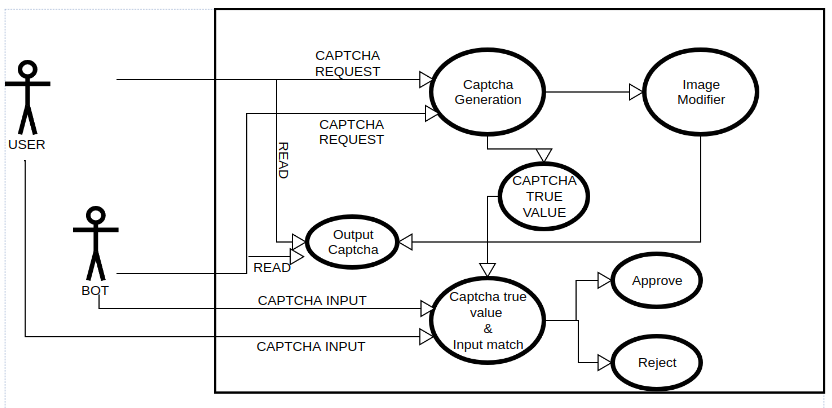
\includegraphics[width=4in]{UML2-PROJECT.png}
    \caption{Model Diagram}
   % \label{fig:my_label}
\end{figure}
\end{frame}
\begin{frame}{Proposed System}
\begin{itemize}
    \item \textbf{Captcha Generation :} A captcha generator is used to  give an input captcha to the system. The captcha consists of 6 characters in text format.
    \item \textbf{Image Modification :} This is where adversarial noise is added to the image using FGSM. The modified image will be indistinguishable to human eye.
    
\end{itemize}

\end{frame}

\begin{frame}{Proposed System}
    \begin{itemize}
    \item \textbf{CNN Model :} Modified image is given to a Convolutional Neural Network model and prediction is made.
Predicted value is compared with the original value and
performance of system is evaluated.
        \item \textbf{Output : }Output is a modified captcha image, which is indistinguishable to
human eye, but wrongly predicted by the CNN model.

    \end{itemize}
\end{frame}

\begin{frame}{Proposed System}
\begin{figure}
    \centering
    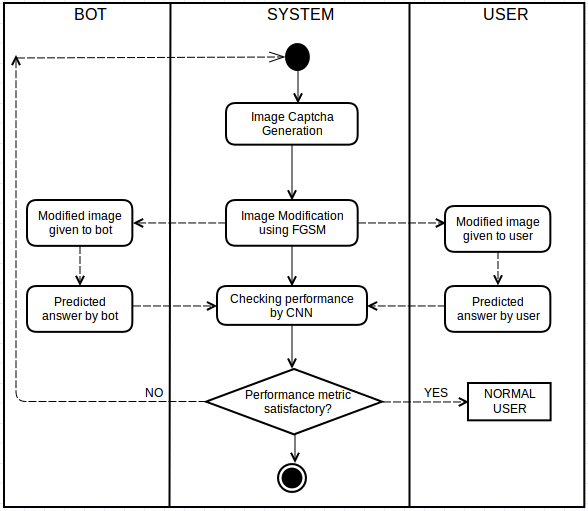
\includegraphics[width=3in]{activity.png}
    \caption{Activity Diagram}
   % \label{fig:my_label}
\end{figure}
\end{frame}

\section{Requirements}

\begin{frame}{Physical Environment}
	\begin{itemize}
	    
	    \item We will train our model in cloud
	    
	    \item Require a programming environment which support TensorFlow framework and allows GPU training
	    
	   
	    
	\end{itemize}
\end{frame}

\begin{frame}{Interfaces}
	\begin{itemize}
	    
	    \item The user will be given a web application to interact with.
	    
	    \item The web application will provide the user with a random captcha generated real time.
	    
	    \item The user will be given a text box to give the response to the displayed captcha. 
	    
	\end{itemize}
\end{frame}

\begin{frame}{Users}
	\begin{itemize}
	    
	    \item The system can be used by an individual or organization who wants to secure their image from image recognition.
	    
	    \item The user will only have to provide the data or dataset on which attack has to be performed on.
	    
	\end{itemize}
\end{frame}


\begin{frame}{Process Constraints}
    \begin{itemize}
	    
	    \item CNN model used for the process has to be trained to recognize the characters from an image captcha close to optimal bayes error.
	    
	    \item Training a CNN model is a difficult task as it requires a lot of computational power which can be harnessed with the help of Cloud GPU .
	      
	\end{itemize}            
\end{frame}
\begin{frame}{Quality Constraints}
\begin{itemize}
    \item Training requires high computational power.
    \item The probability of the randomly guessing each character of the captcha is $ (\frac{1}{26})^6 $ .
    \item This comes out to be about $ 4 \% $ probability ( $ \frac{1}{26} $ )  on individual characters.
    \item As the model used predicts individual character rather than the captcha as a whole.
    \item The attack will be successful if the model's accuracy can be reduced to a number close to $ 4 \%$. 
\end{itemize}
\end{frame}
\section{Project Plan}
\begin{frame}{Project Plan}
\begin{figure}
    \centering
    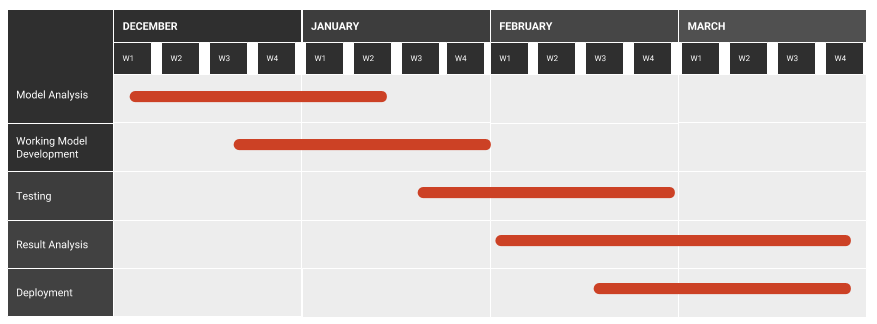
\includegraphics[width=4.5in]{chart.png}
    \caption{Project Plan}
    %\label{fig:my_label}
\end{figure}
\end{frame}

\section{Conclusion}
\begin{frame}{Conclusion}
\begin{itemize}
    \item In the world of existing advanced AI, there exists a security threat as mentioned
    \item Through the proposed implementation of this project, a valid solution can be achieved.
\end{itemize}

\end{frame}


\section{References}

\begin{frame}{References}

  \bibliography{demo}
  \bibliographystyle{abbrv}
\footnotesize{
\begin{thebibliography}{99}

\bibitem[Ian J. Goodfellow, Jonathon Shlens & Christian Szegedy, 2015]{p1}Ian J. Goodfellow, Jonathon Shlens & Christian Szegedy (2015)
\newblock \emph{"Explaining And Harnessing Adversarial Examples"}

\bibitem[Gamaleldin F. Elsayed, Ian Goodfellow, Jascha Sohl-Dickstein , 2018]{p1}Gamaleldin F. Elsayed, Ian Goodfellow, Jascha Sohl-Dickstein  (2018)
\newblock \emph{"Adversarial Reprogramming of Neural Networks"}

\bibitem[F. Tramèr et al. , 2017]{p1} F. Tramèr et al. (2017)
\newblock \emph{“Ensemble Adversarial Training: Attacks and
Defenses” }

\bibitem[Hassan Gomaa, 2011]{p1}Hassan Gomaa (2011)
\newblock \emph{"Software Modelling And Design-UML, Use Cases, Patterns, and
Software Architectures"}
\end{thebibliography}
}

\end{frame}

\end{document}
